% Fig. 1 of the Computational Urban Science version: the architecture diagram as a separate vector file.
% Built by planarena/paper.py (tectonic) into paper/cus/figures/Fig1.pdf. Lettering in a sans-serif font, 8-9 pt.
\documentclass[border=2pt]{standalone}
\usepackage{fontspec}
\setmainfont{texgyreheros}[Extension=.otf, UprightFont=*-regular, BoldFont=*-bold, ItalicFont=*-italic, BoldItalicFont=*-bolditalic]
\usepackage{tikz}
\usetikzlibrary{arrows.meta,positioning,calc}
\begin{document}
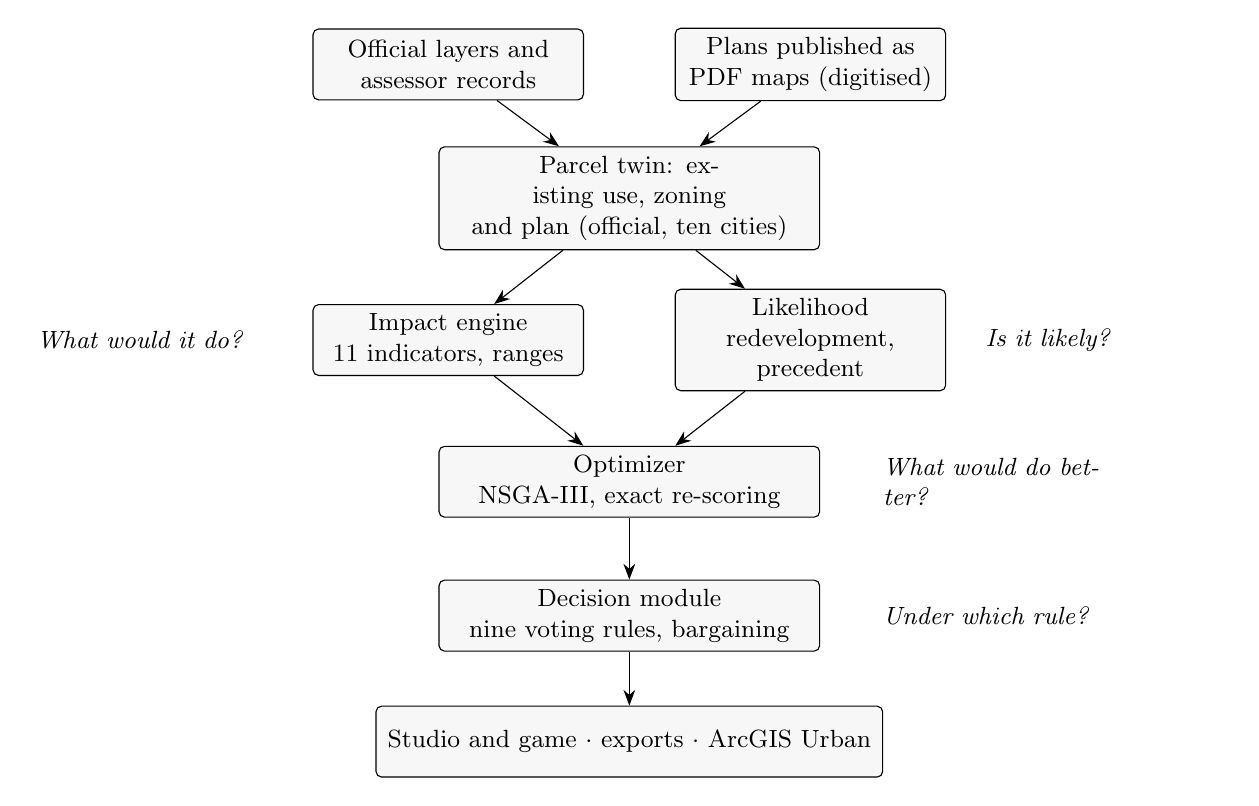
\begin{tikzpicture}[every node/.style={font=\small, align=center},
  box/.style={draw, rounded corners=2pt, minimum height=9mm, text width=32mm, fill=gray!6},
  q/.style={font=\small\itshape, text width=30mm, align=left},
  arr/.style={-{Stealth[length=2mm]}}]
\node[box] (src) at (-2.3, 0) {Official layers and\\assessor records};
\node[box] (pdf) at (2.3, 0) {Plans published as\\PDF maps (digitised)};
\node[box, text width=46mm] (twin) at (0, -1.7) {Parcel twin: existing use, zoning\\and plan (official, ten cities)};
\node[box] (imp) at (-2.3, -3.5) {Impact engine\\11 indicators, ranges};
\node[box] (lik) at (2.3, -3.5) {Likelihood\\redevelopment, precedent};
\node[box, text width=46mm] (opt) at (0, -5.3) {Optimizer\\NSGA-III, exact re-scoring};
\node[box, text width=46mm] (dec) at (0, -7.0) {Decision module\\nine voting rules, bargaining};
\node[box, text width=62mm] (ui) at (0, -8.6) {Studio and game $\cdot$ exports $\cdot$ ArcGIS Urban};
\node[q, anchor=east] at (-4.4, -3.5) {What would it do?};
\node[q, anchor=west] at (4.4, -3.5) {Is it likely?};
\node[q, anchor=west] at (3.1, -5.3) {What would do better?};
\node[q, anchor=west] at (3.1, -7.0) {Under which rule?};
\draw[arr] (src) -- (twin); \draw[arr] (pdf) -- (twin);
\draw[arr] (twin) -- (imp); \draw[arr] (twin) -- (lik);
\draw[arr] (imp) -- (opt); \draw[arr] (lik) -- (opt);
\draw[arr] (opt) -- (dec); \draw[arr] (dec) -- (ui);
\end{tikzpicture}
\end{document}
